\documentclass[]{book}
\usepackage{lmodern}
\usepackage{amssymb,amsmath}
\usepackage{ifxetex,ifluatex}
\usepackage{fixltx2e} % provides \textsubscript
\ifnum 0\ifxetex 1\fi\ifluatex 1\fi=0 % if pdftex
  \usepackage[T1]{fontenc}
  \usepackage[utf8]{inputenc}
\else % if luatex or xelatex
  \ifxetex
    \usepackage{mathspec}
  \else
    \usepackage{fontspec}
  \fi
  \defaultfontfeatures{Ligatures=TeX,Scale=MatchLowercase}
\fi
% use upquote if available, for straight quotes in verbatim environments
\IfFileExists{upquote.sty}{\usepackage{upquote}}{}
% use microtype if available
\IfFileExists{microtype.sty}{%
\usepackage{microtype}
\UseMicrotypeSet[protrusion]{basicmath} % disable protrusion for tt fonts
}{}
\usepackage[margin=1in]{geometry}
\usepackage{hyperref}
\hypersetup{unicode=true,
            pdftitle={Sentinel Asia Handbook},
            pdfauthor={Firman Hadi, Syams Nashrrullah, Ayeisha Sheldon and Dan Tran},
            pdfborder={0 0 0},
            breaklinks=true}
\urlstyle{same}  % don't use monospace font for urls
\usepackage{natbib}
\bibliographystyle{apalike}
\usepackage{longtable,booktabs}
\usepackage{graphicx,grffile}
\makeatletter
\def\maxwidth{\ifdim\Gin@nat@width>\linewidth\linewidth\else\Gin@nat@width\fi}
\def\maxheight{\ifdim\Gin@nat@height>\textheight\textheight\else\Gin@nat@height\fi}
\makeatother
% Scale images if necessary, so that they will not overflow the page
% margins by default, and it is still possible to overwrite the defaults
% using explicit options in \includegraphics[width, height, ...]{}
\setkeys{Gin}{width=\maxwidth,height=\maxheight,keepaspectratio}
\IfFileExists{parskip.sty}{%
\usepackage{parskip}
}{% else
\setlength{\parindent}{0pt}
\setlength{\parskip}{6pt plus 2pt minus 1pt}
}
\setlength{\emergencystretch}{3em}  % prevent overfull lines
\providecommand{\tightlist}{%
  \setlength{\itemsep}{0pt}\setlength{\parskip}{0pt}}
\setcounter{secnumdepth}{5}
% Redefines (sub)paragraphs to behave more like sections
\ifx\paragraph\undefined\else
\let\oldparagraph\paragraph
\renewcommand{\paragraph}[1]{\oldparagraph{#1}\mbox{}}
\fi
\ifx\subparagraph\undefined\else
\let\oldsubparagraph\subparagraph
\renewcommand{\subparagraph}[1]{\oldsubparagraph{#1}\mbox{}}
\fi

%%% Use protect on footnotes to avoid problems with footnotes in titles
\let\rmarkdownfootnote\footnote%
\def\footnote{\protect\rmarkdownfootnote}

%%% Change title format to be more compact
\usepackage{titling}

% Create subtitle command for use in maketitle
\newcommand{\subtitle}[1]{
  \posttitle{
    \begin{center}\large#1\end{center}
    }
}

\setlength{\droptitle}{-2em}

  \title{Sentinel Asia Handbook}
    \pretitle{\vspace{\droptitle}\centering\huge}
  \posttitle{\par}
    \author{Firman Hadi, Syams Nashrrullah, Ayeisha Sheldon and Dan Tran}
    \preauthor{\centering\large\emph}
  \postauthor{\par}
      \predate{\centering\large\emph}
  \postdate{\par}
    \date{2018-09-05}

\usepackage{booktabs}

\usepackage{amsthm}
\newtheorem{theorem}{Theorem}[chapter]
\newtheorem{lemma}{Lemma}[chapter]
\theoremstyle{definition}
\newtheorem{definition}{Definition}[chapter]
\newtheorem{corollary}{Corollary}[chapter]
\newtheorem{proposition}{Proposition}[chapter]
\theoremstyle{definition}
\newtheorem{example}{Example}[chapter]
\theoremstyle{definition}
\newtheorem{exercise}{Exercise}[chapter]
\theoremstyle{remark}
\newtheorem*{remark}{Remark}
\newtheorem*{solution}{Solution}
\begin{document}
\maketitle

{
\setcounter{tocdepth}{1}
\tableofcontents
}
\chapter*{Preface}\label{preface}
\addcontentsline{toc}{chapter}{Preface}

Due to the nature of the Sentinel Asia (SA) works which are related to
disaster response, Value Added Products (VAPs) are expected to be
produced as soon as the data are available. The book serves as a
guidance for streamlining the process and techniques for data processing
related to SA Activities. Hence, it is expected that the book will help
in reaching the objective.

\chapter{Preparation}\label{preparation}

To conduct Sentinel Asia activities, there are several things that need
to be prepared, (1) Hardware, (2) softwares and (3) Standard Operational
Procedures.

\section{Hardwares}\label{hardwares}

There are three main computers used for Sentinel Asia works, (1) CentOS
Linux , (2) Windows PC and (3) MacPro. CentOS Linux is used as Image
Management System, activating scripts for PDAN website and serve as data
storage downloaded from Sentinel Asia website. Since we will not
continue to use PDAN website, CentOS Linux can be develop as the server
for crowdsourcing or field validation by implementing DRMSurvey or
Ushahidi for example. Windows PC is used to handle processing data
related to flood, while MacPro is used to process data related to
geological hazard such as volcano and earthquake.

\section{Softwares}\label{softwares}

The main softwares for processing data can be divided to proprietary and
open source sofwares. ArcGIS and ENVI are main proprietary sofwares
used, while for open source softwares, QGIS, SNAP and GMT5SAR are
utilized.

\section{Standard Operational
Procedures}\label{standard-operational-procedures}

Standard Operational Procedures (SOP) is the main procedure develop for
each type of disasters. The main objective of writing this SOP is to
standardize the process, so anyone can do the process with the same
output or result.

\chapter{Introduction}\label{intro}

Sentinel Asia is a voluntary initiative to provide satellite data at a
time of a disaster, and to coordinate support in collaboration with data
provider nodes (DPNs), data analysis nodes (DANs), and disaster
management organizations (DMOs) in the Asia-Pacific region. Data
analyses and value added product (VAP) generation is done through
several agencies including the GIC/AIT, which is the Primary Data
Analysis Node (P-DAN). Moreover, Sentinel Asia also supports activities
on disaster risk reduction (DRR) to its member countries in the region.
In this respect, technical and disaster management organizations are
members of Sentinel Asia and are known as joint project team members
(JPTM).

The time lapse of work-flow from a disaster occurrence to the product
delivery stage is an important factor that has a high impact on DRR
activities. The work-flow is a process chain consisting of various
stages such as an emergency observation request (EOR), Sentinel Asia
activation, satellite observations, image processing and analyses,
value-added product (VAPs) generation, product delivery and sharing. It
is important to reduce the time gaps in this process chain. The GIC/AIT
has provided the service as the P-DAN during the contract period.

The main components of the works are (1) the Project Manager (PM)
activities of the International Disaster Charter (IDC) and (2)
generation, provision and evaluation of Value Added Products (VAPs).

All the service for Sentinel Asia activation is provided by effectively
communicating with the Sentinel Asia Secretariat and collecting related
information in order to identify the severity and to monitor the
progress after an activation. Assistance is provided to the authorized
users (AU) of the Asian Disaster Reduction Center (ADRC) member
countries to receive data and products in a timely manner and to share
VAPs with the ADRC and its member countries. After the VAPs are
generated, close communication is maintained during the contract period
with DAN members of the Sentinel Asia-activated countries.

\section{Project Manager (PM) Activities of International Disaster
Charter
(IDC)}\label{project-manager-pm-activities-of-international-disaster-charter-idc}

When a major disaster occurs, the Asian Disaster Reduction Center (ADRC)
can escalate a Sentinel Asia emergency observation request to the
International Disaster Charter (IDC). A project manager (PM), such as
the GIC/AIT, will be nominated from relevant national agencies or
international organizations. The PM role is to ensure effective
communication between the data providers or partner agencies (PA), value
added companies/resellers and authorized users (AU). The PM will
coordinate the activation, ensuring that the acquisition of satellite
images is under way, managing the generation of products or information,
and making sure that the products are delivered to the users according
to their needs and expectations. The Charter activation is considered
closed 30 days after the initial activation date or when the end users
have enough products for their requirements. The PM will then have to
submit a report to the Charter Executive Secretariat (the member of the
PA that nominated the PM -- in this case the JAXA) - within 45 days of
the initial activation date through email or the COS-2 system. The PM
report will conclude the PM's work for this Charter activation.

\section{Sentinel Asia Activities}\label{sentinel-asia-activities}

As the primary data analysis node (P-DAN) of Sentinel Asia, the GIC/AIT
has been effectively communicating with the Sentinel Asia
Secretariat/ADRC and coordinating the response of DAN members for each
emergency observation request. The GIC/AIT analyzed satellite data which
provided by the data provider nodes (DPNs), and then created VAPs and
shared such satellite-based disaster information products to end users
in timely manner.

\chapter{Sentinel Asia Activation Response
Workflow}\label{sentinel-asia-activation-response-workflow}

Here is a the general procedure that should be followed during the
Sentinel Asia Activation.

\section{Immediate Response}\label{immediate-response}

\subsection{Work management}\label{work-management}

\begin{enumerate}
\def\labelenumi{\arabic{enumi}.}
\tightlist
\item
  Create an activation folder in Kepler
\item
  Track the observation plan of satellite data
\end{enumerate}

\subsection{Initial communication with requestor/end
user}\label{initial-communication-with-requestorend-user}

\begin{enumerate}
\def\labelenumi{\arabic{enumi}.}
\tightlist
\item
  Confirm the affected areas
\item
  Update the most recent ground situation
\item
  Identify the user needs of VAPs
\item
  Request the user to share ground information
\end{enumerate}

\subsection{Download/preparing vector
data}\label{downloadpreparing-vector-data}

The data for many of Asian countries have been prepared in ArcGIS
Geodatabase. Please see Appendices to see how to connect to the
Geodatabase.

\subsection{Download other relevant
data}\label{download-other-relevant-data}

\begin{enumerate}
\def\labelenumi{\arabic{enumi}.}
\tightlist
\item
  Download SRTM
\item
  Download WorldPop
\end{enumerate}

\subsection{Initial data processing}\label{initial-data-processing}

\begin{enumerate}
\def\labelenumi{\arabic{enumi}.}
\tightlist
\item
  Create project in ArcGIS Pro
\item
  Connect to the Country DataBase
\item
  Identify the affected admin area
\item
  Calculate slope from DEM
\end{enumerate}

\subsection{ArcGIS Online}\label{arcgis-online}

\begin{enumerate}
\def\labelenumi{\arabic{enumi}.}
\tightlist
\item
  Create a project for the activation
\item
  Create a rainfall monitoring tab
\item
  Create a tab for social media integration
\end{enumerate}

\subsection{PDAN System}\label{pdan-system}

\begin{enumerate}
\def\labelenumi{\arabic{enumi}.}
\tightlist
\item
  Activate email notification
\item
  Update PDAN website (front page)
\item
  Create PDAN forum
\item
  Integrate ArcGIS Online
\end{enumerate}

\subsection{Prepare activation report (using
template)}\label{prepare-activation-report-using-template}

\begin{enumerate}
\def\labelenumi{\arabic{enumi}.}
\tightlist
\item
  Write `Overview'
\item
  Write `Description of Disaster Situation'
\item
  Write `Disaster Affected Areas'
\item
  Write `Data Availability'
\item
  Write `Communication'
\end{enumerate}

\section{Data provision and VAP
generation}\label{data-provision-and-vap-generation}

\subsection{Work management}\label{work-management-1}

\begin{enumerate}
\def\labelenumi{\arabic{enumi}.}
\tightlist
\item
  Call for a meeting, if necessary
\item
  Assign staffs available for data processing
\end{enumerate}

\subsection{Communication with
requestor/end-user}\label{communication-with-requestorend-user}

\subsubsection{Check and re-check}\label{check-and-re-check}

Check the draft of VAP by overlaying it with OpenStreetMap data or other
GIS services (Google etc.)

\chapter{PC/Servers Management}\label{pcservers-management}

For Sentinel Asia and IDC Activation, we use several PC and servers for
processing, storing data and results.

\section{ArcGIS Enterprise Geodatabase
Connection}\label{arcgis-enterprise-geodatabase-connection}

\subsection{Downloading SQL Server and setting it
up}\label{downloading-sql-server-and-setting-it-up}

Note: This needs to be completed only once before you can connect to the
server.

\begin{enumerate}
\def\labelenumi{\arabic{enumi}.}
\tightlist
\item
  Download and install SQL sever
\item
  This is found in KEPLA:
  \textbackslash{}203.159.29.17\Kepler\C-Resources\E-Software\_and\_Tools\arcgis\_server
\end{enumerate}

\begin{center}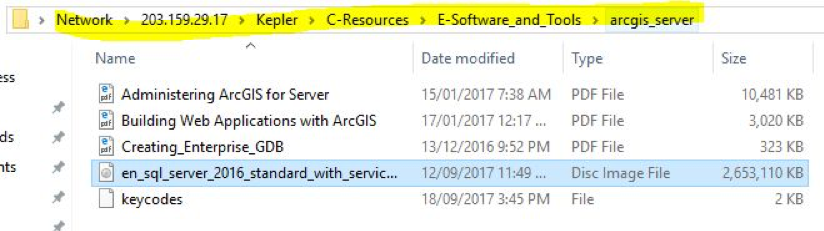
\includegraphics[width=0.7\linewidth]{img/fig43_arcgis1} \end{center}

\begin{center}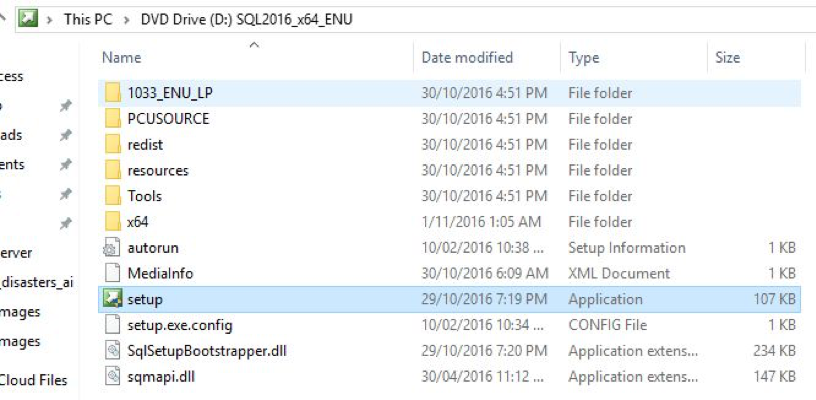
\includegraphics[width=0.7\linewidth]{img/fig43_arcgis2} \end{center}

\begin{enumerate}
\def\labelenumi{\arabic{enumi}.}
\setcounter{enumi}{2}
\tightlist
\item
  Go through general installation prompts to install.
\end{enumerate}

\begin{center}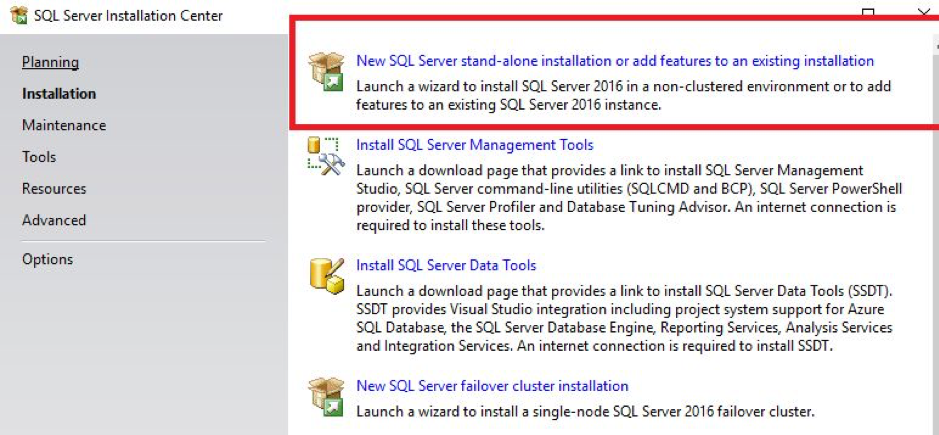
\includegraphics[width=0.7\linewidth]{img/fig43_arcgis3} \end{center}

\begin{enumerate}
\def\labelenumi{\arabic{enumi}.}
\setcounter{enumi}{3}
\tightlist
\item
  Click next and agree to go through the installation steps.
\item
  Features selection -select the boxes shown below
\end{enumerate}

\begin{center}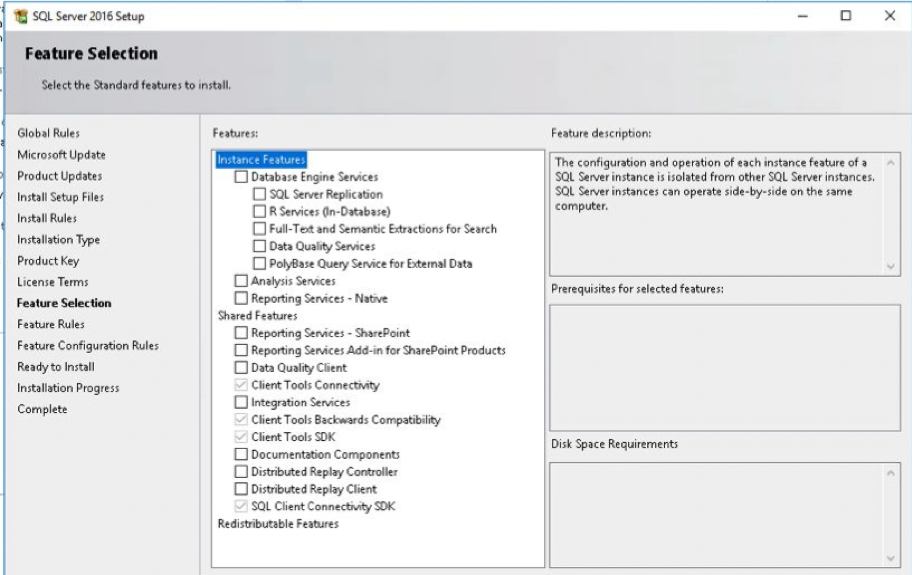
\includegraphics[width=0.7\linewidth]{img/fig43_arcgis4} \end{center}

\begin{enumerate}
\def\labelenumi{\arabic{enumi}.}
\setcounter{enumi}{5}
\tightlist
\item
  Complete the rest of the steps and instal the server.
\end{enumerate}

\subsection{Connecting to
Geodatabases}\label{connecting-to-geodatabases}

Connecting to the server and the databases is important as it allows the
user to find and locate common data.

You can connect through either ArcCatalog or ArcGIS Pro Contents.
Connecting through ArcCatalog:

\begin{enumerate}
\def\labelenumi{\arabic{enumi}.}
\item
  Open ArcCatalog
\item
  Add Database connection as follows:
\end{enumerate}

\begin{center}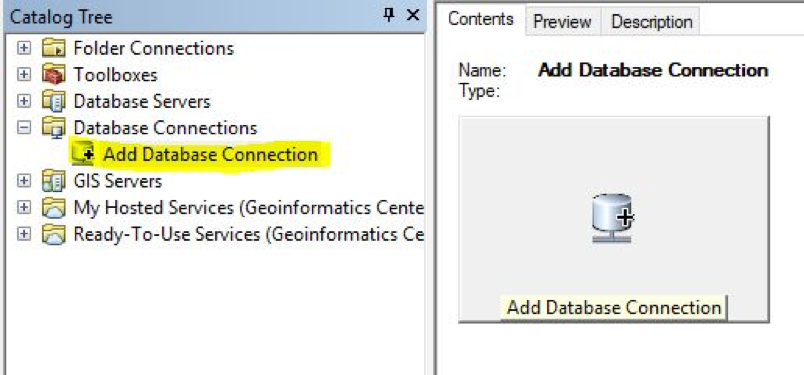
\includegraphics[width=0.7\linewidth]{img/fig43_arcgis5} \end{center}

\begin{enumerate}
\def\labelenumi{\arabic{enumi}.}
\setcounter{enumi}{2}
\tightlist
\item
  Connect to the Database using the following fields:
\end{enumerate}

\begin{figure}

{\centering 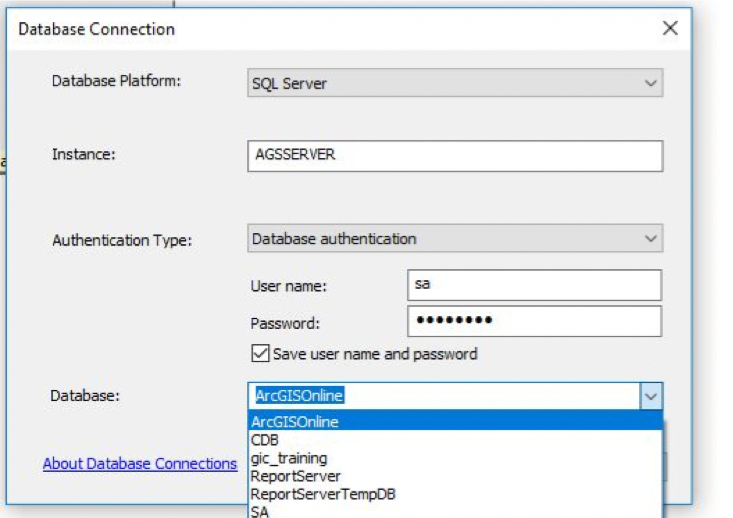
\includegraphics[width=0.7\linewidth]{img/fig43_arcgis6} 

}

\caption{Username: gic, password: GICuser123}\label{fig:fig411f}
\end{figure}

\begin{enumerate}
\def\labelenumi{\arabic{enumi}.}
\setcounter{enumi}{3}
\tightlist
\item
  On the Database drop down list, here is where you select which
  database to connect to. Perform this step multiple times to connect to
  all relevant databases you want to access - once connected you won't
  need to connect again.
\end{enumerate}

Databases:

\begin{itemize}
\item
  CDB - This is the common database with all common country data
  (vector)
\item
  CDB\_R - This it the common database with all raster data
\item
  ArcGIS online - This is for ArcGIS Online files
\item
  SA - Sentinel Asia
\item
  SA\_R - Sentinel Asia Raster
\end{itemize}

\begin{center}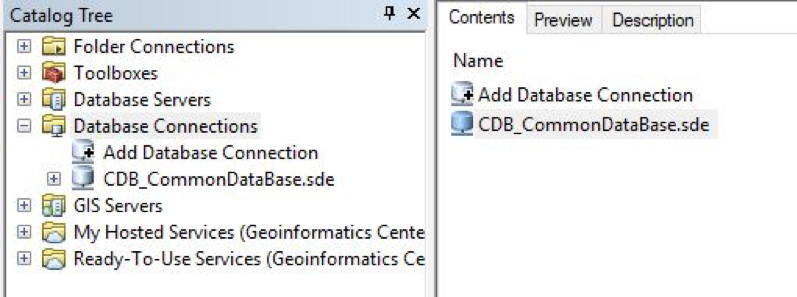
\includegraphics[width=0.7\linewidth]{img/fig43_arcgis7} \end{center}

\begin{enumerate}
\def\labelenumi{\arabic{enumi}.}
\setcounter{enumi}{4}
\item
  Once the chosen Database is connected it will show on the side bar, y
  ou can rename this to the database name - double click this to open
  and view the data. All data in the database will show up here, with
  the database name followed by the file name.
\item
  For the common database, all countries are clustered into raster
  datasets, click these to open.
\end{enumerate}

\begin{center}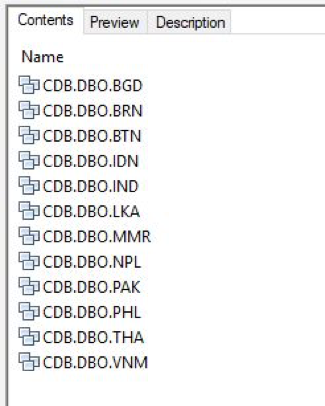
\includegraphics[width=0.4\linewidth]{img/fig43_arcgis8a} \end{center}

\begin{center}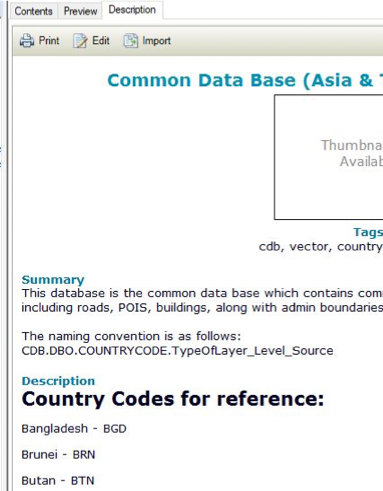
\includegraphics[width=0.4\linewidth]{img/fig43_arcgis8b} \end{center}

Note: Click description to find the corresponding names for country
codes

\begin{center}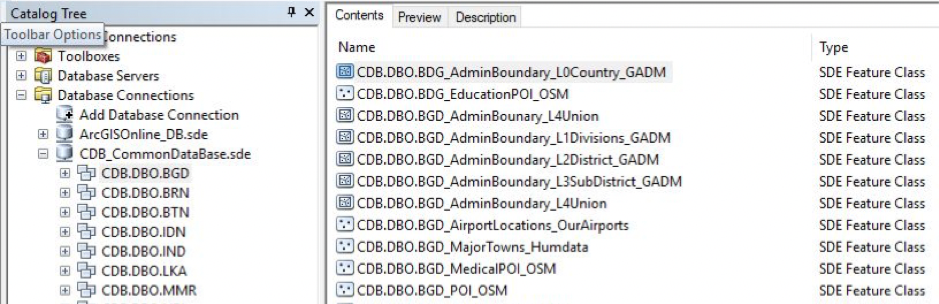
\includegraphics[width=0.7\linewidth]{img/fig43_arcgis9} \end{center}

\begin{enumerate}
\def\labelenumi{\arabic{enumi}.}
\setcounter{enumi}{6}
\tightlist
\item
  If you want to use this data in your map file, just drag the data into
  ArcMap from ArcCatalog, it will open like any file
\end{enumerate}

\begin{center}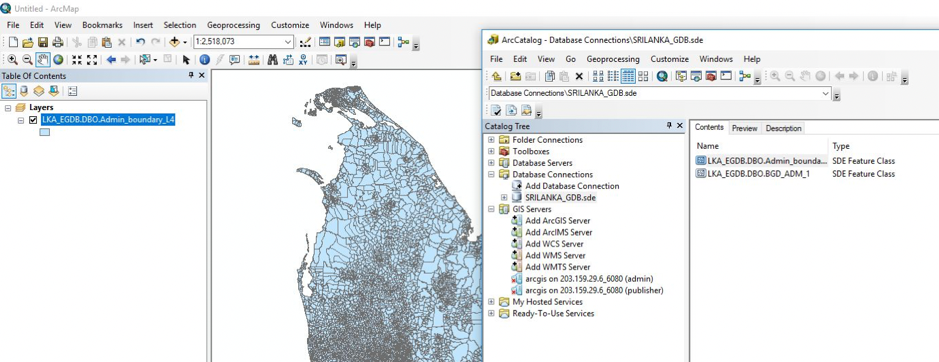
\includegraphics[width=0.7\linewidth]{img/fig43_arcgis10} \end{center}

\begin{enumerate}
\def\labelenumi{\arabic{enumi}.}
\setcounter{enumi}{7}
\tightlist
\item
  You can also access the database from ArcCatalog in the side bar of
  ArcMap:
\end{enumerate}

\begin{center}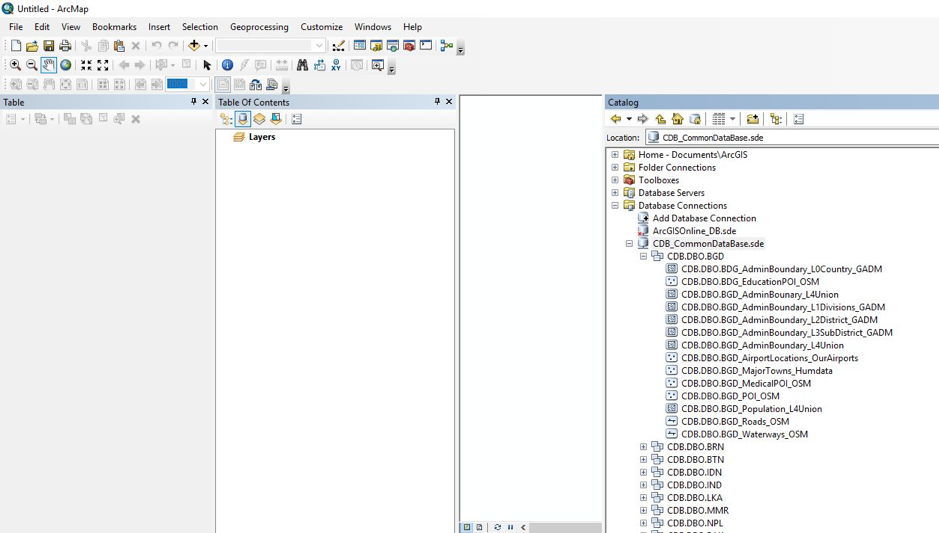
\includegraphics[width=0.7\linewidth]{img/fig43_arcgis11} \end{center}

Following link in Youtube will provide you on the how to do the
procedure \url{https://youtu.be/3DWrBp_5MJc}

\section{SQL Server}\label{sql-server}

GIC Enterprise Databases are stored in SQL Server. The databases are
regularly backup to Kepler and Google Drive (geoinfo )

\subsection{Maintenance}\label{maintenance}

\subsubsection{SQL Backup and
Monitoring}\label{sql-backup-and-monitoring}

\url{https://youtu.be/OBk0SdeB3IM}

\subsubsection{SQL Database Recovery}\label{sql-database-recovery}

We have to make one session to practice on how to recover database, in
case of hard drive failure.

\section{IMS-Server}\label{ims-server}

\subsection{Connection}\label{connection}

\section{Sentinel-PC}\label{sentinel-pc}

\subsection{Connection}\label{connection-1}

\url{https://www.youtube.com/watch?v=Dpx9NslsIqg\&feature=youtu.be}

\section{MacPro}\label{macpro}

\subsection{Connection}\label{connection-2}

\url{https://youtu.be/xje9lyKYTSw}

\section{Cloud Server (Google Compute
Engine)}\label{cloud-server-google-compute-engine}

In case of IDC activation, some of the data will be provided through FTP
sites (port 21). FTP port is restricted at the office network, we have
to download the data by using the server located in GIC Google Compute
Engine. This method will also increase downloading speed from certain
data provider (e.g., CNES).

The method is explained in this video link
\url{https://youtu.be/NS6oLCNrGHg}

\chapter{Standard Operational Procedure
(SOP)}\label{standard-operational-procedure-sop}

This chapter is arranged to different sections according to the most
frequent type of disaster in previous Sentinel Asia Activities. On each
section, the explanation will be based on available data.

\section{Data Download}\label{data-download}

\subsection{Sentinel Asia Website}\label{sentinel-asia-website}

\url{https://youtu.be/yZJi4FRw4Ps}

\subsection{IDC Data Download via FTP}\label{idc-data-download-via-ftp}

Data can be downloaded from Google Cloud Compute Engine via FTP and put
in HTTP folder.

\section{Data processing}\label{data-processing}

\subsection{Flood}\label{flood}

\subsubsection{SAR}\label{sar}

\paragraph{ArcGIS}\label{arcgis}

Before processing the data, it is better to check the processing level
from the filename.

The data (pre and post flood) was processed through 5 main steps: (1)
Data processing including: Radiometric calibration, Speckle filtering,
and Coordinate transformation; (2) Image differencing using image pre
and post-flood; (3) Thresholding of backscatter changes; (4) Image
filtering using majority filter; and (5) Mapping of flooded area. The
methodology is shown in the figure below.

Image for Workflow

\begin{figure}

{\centering 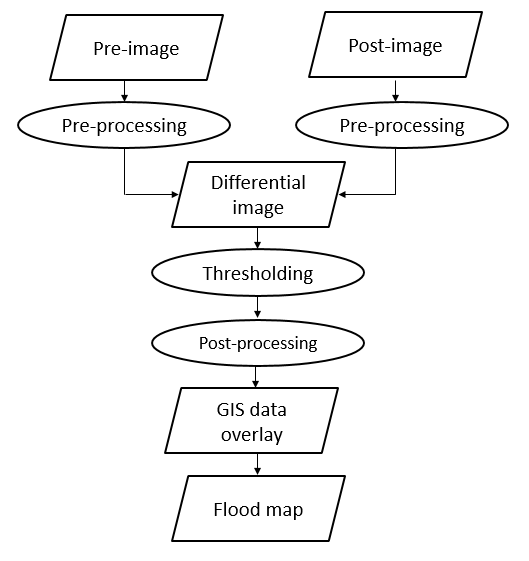
\includegraphics[width=0.7\linewidth]{img/fig41_workflow} 

}

\caption{Flood Detection General Workflow}\label{fig:fig42a}
\end{figure}

(Step 1: ArcGIS Pro) Radiometric calibration, Speckle filtering, and
Coordinate transformation

Raster Function in ArcGIS Pro is used to process the images (pre and
post-flood), with flowchart as follow:

\begin{figure}

{\centering 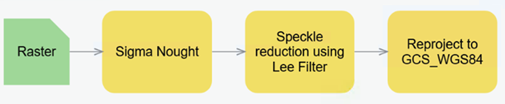
\includegraphics[width=0.7\linewidth]{img/fig41_workflow1} 

}

\caption{ALOS-2 radiometric and geometric calibration Workflow}\label{fig:fig42b}
\end{figure}

\begin{itemize}
\tightlist
\item
  To convert raw image to sigma nought with the formula 20 * Log10(DN)
  -- 83
\end{itemize}

\begin{figure}

{\centering 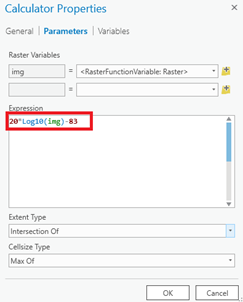
\includegraphics[width=0.7\linewidth]{img/fig41_workflow2} 

}

\caption{ALOS-2 radiometric calibration formula}\label{fig:fig42c}
\end{figure}

\begin{itemize}
\tightlist
\item
  To do image filtering with Lee filter (5x5 window size).
\end{itemize}

\begin{figure}

{\centering 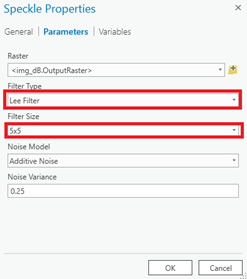
\includegraphics[width=0.7\linewidth]{img/fig42_workflow3} 

}

\caption{ALOS-2 speckle reduction}\label{fig:fig42d}
\end{figure}

\begin{itemize}
\tightlist
\item
  To convert coordinate to GCS\_WGS\_1984
\end{itemize}

\begin{figure}

{\centering 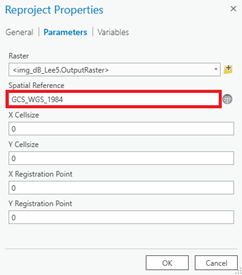
\includegraphics[width=0.7\linewidth]{img/fig42_workflow4} 

}

\caption{Reprojection to GCS WGS84}\label{fig:fig42e}
\end{figure}

(Step 2: ArcGIS Pro) Image differencing Using the Calculator raster
function to create a difference image, with the formula Change =
(Post-flood) - (Pre-flood)

\begin{figure}

{\centering 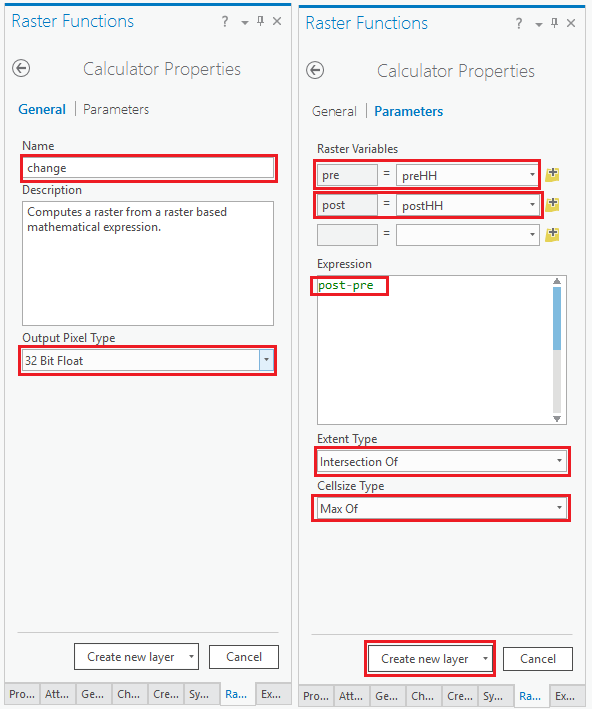
\includegraphics[width=0.7\linewidth]{img/fig42_workflow5} 

}

\caption{Image differencing}\label{fig:fig42f}
\end{figure}

(Step 3: ArcGIS Pro) Thresholding of backscatter changes Using the
Calculator raster function to extract flood inundation areas from the
result in step 2 with threshold \textless{} -3.

\begin{figure}

{\centering 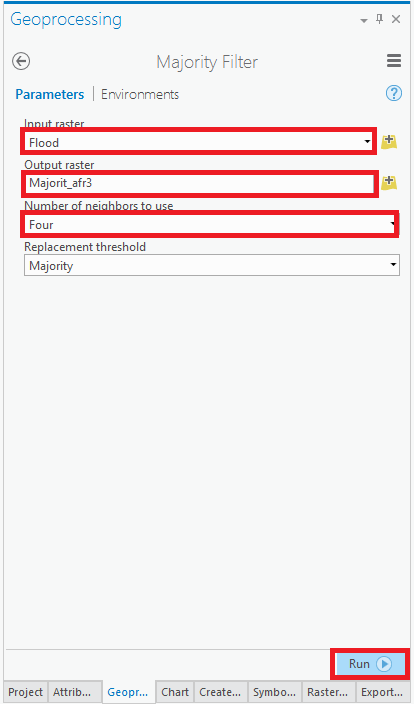
\includegraphics[width=0.7\linewidth]{img/fig42_workflow6} 

}

\caption{Image thresholding}\label{fig:fig42g}
\end{figure}

(Step 4: ArcGIS Pro) Image filtering Majority filter is applied to
reduce noise (salt and pepper) from result in step 3.
(Toolboxes\Spatial Analyst Tools\Generalization\Majority Filter)

\begin{figure}

{\centering 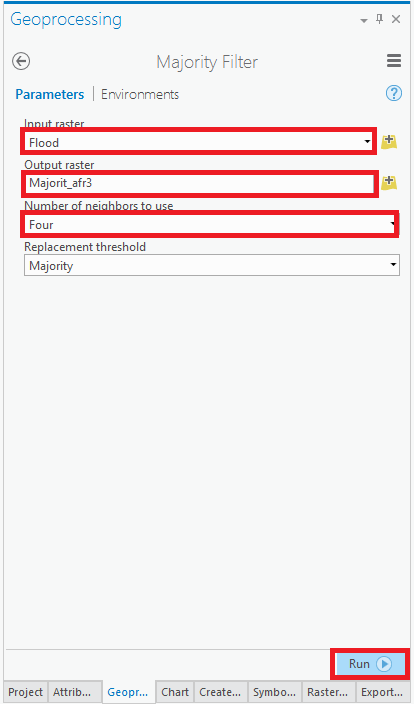
\includegraphics[width=0.7\linewidth]{img/fig42_workflow6} 

}

\caption{Image filtering}\label{fig:fig42h}
\end{figure}

Then, convert raster to polygon and export to shapefile (.shp) format
for a further step in ArcMap.

\paragraph{QGIS}\label{qgis}

Flood detection can be carried out in QGIS by using Graphical Modeling
as shown in the following video

\url{https://youtu.be/HR_7kENFGT4}

\subsubsection{Optical data}\label{optical-data}

\subsubsection{Google Earth Engine (GEE)}\label{google-earth-engine-gee}

// Load Sentinel-1 images to map the flooding area, // This script was
originally written by Simon Ilyushchenko (GEE team) // Default location
var pt = ee.Geometry.Point(96.4633,17.79); //, , Grand Morin near
Coulommiers

// Load Sentinel-1 C-band SAR Ground Range collection (log scaling, VV
co-polar, Descending) var collection =
ee.ImageCollection(`COPERNICUS/S1\_GRD').filterBounds(pt).
filter(ee.Filter.listContains(`transmitterReceiverPolarisation', `VV')).
filter(ee.Filter.eq(`orbitProperties\_pass', `DESCENDING')).
select(`VV');

// Filter by date, ensure that the result will cover only 1 day

var before = collection.filterDate(`2016-05-5', `2016-05-6').mosaic();
var after = collection.filterDate(`2018-07-24', `2018-07-25').mosaic();

// Threshold smoothed radar intensities to identify ``flooded'' areas.
var SMOOTHING\_RADIUS = 100; var DIFF\_UPPER\_THRESHOLD = -3; var
diff\_smoothed = after.focal\_median(SMOOTHING\_RADIUS, `circle',
`meters') .subtract(before.focal\_median(SMOOTHING\_RADIUS, `circle',
`meters')); var diff\_thresholded =
diff\_smoothed.lt(DIFF\_UPPER\_THRESHOLD);

//Define the extent for exporting the result var geometry =
ee.Geometry.Rectangle({[}105.321, 20.3574, 106.971, 21.313473{]});

// Display map Map.centerObject(pt, 10); Map.addLayer(before,
\{min:-30,max:0\}, `Before flood'); Map.addLayer(after,
\{min:-30,max:0\}, `After flood'); Map.addLayer(after.subtract(before),
\{min:-10,max:10\}, `After - before', 0); Map.addLayer(diff\_smoothed,
\{min:-10,max:10\}, `diff smoothed', 0);
Map.addLayer(diff\_thresholded.updateMask(diff\_thresholded),
\{palette:``0000FF''\},`flooded areas - blue',1);

// Export the image, specifying scale and region.

// Pre-flood Export.image.toDrive(\{ image: before, description:
`MMM\_image\_SentinelBefore', scale: 30, region: geometry \});

// Post-flood

Export.image.toDrive(\{ image: after, description:
`MMM\_image\_SentinelAfter', scale: 30, region: geometry \});

//Flood Export.image.toDrive(\{ image: diff\_thresholded, description:
`MMM\_image\_SentinelFlood', scale: 30, region: geometry \});

\subsubsection{Permanent Water}\label{permanent-water}

\subsection{Earthquake}\label{earthquake}

\begin{enumerate}
\def\labelenumi{\arabic{enumi}.}
\item
  Connect to MacPro by using VNC Viewer. Username and password to
  connect will be provided separately.
\item
  Create folder with the structure as below :
\item
  IND

  \begin{enumerate}
  \def\labelenumii{\arabic{enumii}.}
  \tightlist
  \item
    raw folder
  \item
    topo folder
  \item
    config.alos2.slc.txt (configuration file for running the process)
  \end{enumerate}
\item
  Download DEM from GMTSAR website
\item
  Go to this link \url{http://topex.ucsd.edu/gmtsar/demgen/}
\item
  Enter the coordinate for north, south, east and west. The boundary
  cannot span more than 4 longitude by 4 latitude degrees.
\item
  Click Generate to process.
\item
  If it has finished, click Download to get the result.
\item
  \begin{figure}
  \centering
  \includegraphics{https://d2mxuefqeaa7sj.cloudfront.net/s_16280D51B2B6313EEF06D7EC9BB498F0F653DE3F6FC0EF0F53F10752E0108E06_1534493067726_Screen+Shot+2018-08-17+at+14.26.27.png}
  \caption{}
  \end{figure}
\item
  Copy the ALOS-2 data (IMG, LED and VOL- files) to raw folder
\item
  Extract the files downloaded from DEM Generation process in GMTSAR
  website and copy all of the files to topo folder.
\item
  Modify the config\_alos2\_slc.txt file
\item
  If it is the first time in processing, set the value for proc\_stage
  to 1 (proc\_stage = 1).
\item
  Set dummy value for SLC\_factor, 4.0 (SLC\_factor = 4.0). This is
  important as we will receive a warning message to change the value to
  the correct one.
\item
  Set topo\_phase to 1, to subtract topo\_ra from the phase (topo\_phase
  = 1)
\item
  Set shift\_topo to 0.
\item
  Set switch\_master to 1 if we assume master as repeat and slave as
  reference. Set it to 0, if we assume master as reference and slave
  image as repeat. The default value is 0 (switch\_master = 0)
\item
  For filtering, set filter\_wavelength = 100, and filter1 =
  gauss\_alos\_100m.
\item
  Set decimation of images to 1 if we want higher resolution image and
  set it to 2 if we want smaller resolution (dec\_factor = 1)
\item
  Set correlation threshold for snapu to 0.1 (threshold\_snaphu = 0.1)
\item
  Leave the option blank to unwrap the whole region (region\_cut = ).
  Note that, in the latest version of GMT5SAR, this option will be
  executed if we write the config for interpolation (near\_interp = 1).
  If we don't put this option for interpolation, the result will be
  unwrapped to half of the image.
\item
  For masking the Lake or Ocean, set switch\_land to 1 (switch\_land =
  1).
\item
  Set defomax = 0 for smoother unwrapped phase.
\item
  Set threshold\_geocode = .10
\item
  Under IND folder, by using Command Line, run this command
  ``p2p\_ALOS2\_SLC.csh IMG-master IMG-slave config.alos2.slc.txt''.
  Change IMG-master with the full file name of IMG as master and
  IMG-slave with the full file name of slave IMG.
\item
  Wait for the process to finish. It will take some time depend on the
  CPU speed and also the type of data. SM1 data will take longer than
  SM3.
\item
  The results will be created in intf folder, under IND folder.
\item
  KML files can be opened using Google Earth. Files without \_ll suffix
  are still in azimuth and range coordinates, those with \_ll suffix
  mean already in Geographic Coordinate System WGS84.
\item
  Files with .grd extension can be opened using QGIS and then exported
  to GeoTIFF format.
\item
  The results in TIFF extension are used in ArcMap for layouting.
\end{enumerate}

\subsection{Volcano}\label{volcano}

\subsection{Landslide}\label{landslide}

\subsection{Glacier Lake Outburst
Flood}\label{glacier-lake-outburst-flood}

\subsection{Forest Fire}\label{forest-fire}

\section{Data Layout}\label{data-layout}

\subsection{Check and re-check}\label{check-and-re-check-1}

\begin{enumerate}
\def\labelenumi{\arabic{enumi}.}
\tightlist
\item
  Check and re-check the draft of VAP before uploading to SA server.
\item
  Compare the geometry with other available online data \#\# Data Upload
  to Server
\end{enumerate}

\chapter*{Appendices}\label{appendices}
\addcontentsline{toc}{chapter}{Appendices}

\subsection*{ArcGIS Enterprise Geodatabase
connection}\label{arcgis-enterprise-geodatabase-connection-1}
\addcontentsline{toc}{subsection}{ArcGIS Enterprise Geodatabase
connection}

\subsection*{Useful Links}\label{useful-links}
\addcontentsline{toc}{subsection}{Useful Links}

\subsection*{ArcGIS Pro scripts}\label{arcgis-pro-scripts}
\addcontentsline{toc}{subsection}{ArcGIS Pro scripts}

\subsection*{Generalization script}\label{generalization-script}
\addcontentsline{toc}{subsection}{Generalization script}

\bibliography{book.bib,packages.bib}


\end{document}
